\subsection{Rahmen}
\label{subsec:Rahmen}

Der Rahmen besteht aus 20x20mm Aluminium X-Profilen. Diese haben einerseits den Vorteil, dass sie sehr Stabil sind und anderseits sind diese vielseitig einsetzbar. Die Profile verfügen über eine Nut, in welche sogenannte \flqq Nutensteine\frqq~eingesetzt werden. Diese verfügen wiederum über eine Bohrung mit einem Gewinde. Durch diese Kombination kann Mittels Nutenwinkel ein stabiler Rahmen aufgebaut werden. In Abbildung \ref{fig:Rahmen} sind diese Bauteile zu sehen.  

\begin{figure}[H]
	\centering
	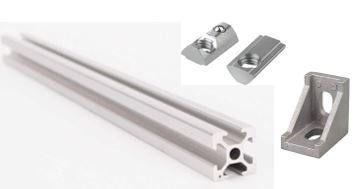
\includegraphics[width=0.5\textwidth]{graphics/Rahmen}
	\caption{Bauteile für den Rahmen des Partymixers}.
	\label{fig:Rahmen}
\end{figure}